%%%%%%%%%%%%%%%%%%%%%%%%%%%%%%%%%%%%%%%%%%
% Engineering problems / LaTeX Template
%		Semester 5
%		Institut d'Optique Graduate School
%%%%%%%%%%%%%%%%%%%%%%%%%%%%%%%%%%%%%%%%%%
%	5N-OptoElec-Sujet	
%%%%%%%%%%%%%%%%%%%%%%%%%%%%%%%%%%%%%%%%%%
%
% Created by:
%	Julien VILLEMEJANE - 05/may/2025
%	
%
%%%%%%%%%%%%%%%%%%%%%%%%%%%%%%%%%%%%%%%%%%
% Professional Newsletter Template
% LaTeX Template
% Version 1.0 (09/03/14)
%
% Created by:
% Bob Kerstetter (https://www.tug.org/texshowcase/) and extensively modified by:
% Vel (vel@latextemplates.com)
% 
% This template has been downloaded from:
% http://www.LaTeXTemplates.com
%
% License:
% CC BY-NC-SA 3.0 (http://creativecommons.org/li censes/by-nc-sa/3.0/)
%
%%%%%%%%%%%%%%%%%%%%%%%%%%%%%%%%%%%%%%%%%

\documentclass[a4paper,11pt,twoside]{book} % The default font size is 10pt; 11pt and 12pt are alternatives

%%%%%%%%%%%%%%%%%%%%%%%%%%%%%%%%%%%%%%%%%%%%%%%%%%%%%%%%%%%%%%%%%%%%%%%%%%%%%%%%%%%%%%%%%%%%%%%%%%%%%%%%%%%%%%%%%%%%%%%%%%%%%%%%%%%%%%%%%%%%%%%%%%%%%%%%%%%%%%%%%%%%%%%%%%%%%%%%%%%%%%%%%%%%%%%%%%%%%%%%%%%%%%%%%%%%%%%%%%%%%%%%%%%%%%%%%%%%%%%%%%%%%%%%%%%%
\usepackage{opto_elec_villemejane}

%%%%%%%%%%%%%%%%%%%%%%%%%%%%%%%%%%%%%%%%%%%%%%%%
%%%%%%%%%%%%%%%%%%%%%%%%%%%%%%%%%%%%%%%%%%%%%%%%
%%%%%%%%%%%%%%%%%%%%%%%%%%%%%%%%%%%%%%%%%%%%%%%%
%%%%%%%%%%%%%%%%%%%%%%%%%%%%%%%%%%%%%%%%%%%%%%%%
\begin{document}



% Page de garde
\begin{titlepage}

\begin{center}
	\begin{minipage}{2.5cm}
	\begin{center}
		
\includegraphics[width=8cm]{images/LEnsE_IOGS.jpg}
	\end{center}
\end{minipage}\hfill
\begin{minipage}{10cm}
	\begin{center}
	\textbf{Institut d'Optique Graduate School }\\[0.1cm]
    \textbf{TP d'Opto-Électronique}


	\end{center}
\end{minipage}\hfill


\vspace{4cm}


{\huge \bfseries \textsc{Opto-Électronique}} \\[0.5cm]
{\large \bfseries Travaux Pratiques} \\[0.2cm]
Semestre 5

\vspace{2cm}
% Title
\rule{\linewidth}{0.3mm} \\[0.4cm]
{ \huge \bfseries\color{violet_iogs} Développer et caractériser \\ un système de photodétection \\[0.4cm] }
\rule{\linewidth}{0.3mm} \\[1cm]

\vspace{4cm}

% Bottom of the page
%{\textbf{\large {Année universitaire} 2024-2025}}

\textit{Ce sujet est disponible au format électronique sur le site du LEnsE - https://lense.institutoptique.fr/ dans la rubrique Année / Première Année / Opto-Electronique S5 / TP / Sujet.}

\vspace{1cm}

\begin{minipage}{5cm}
\begin{center}

\includegraphics[width=3cm]{./images/logocc}\\
\small
  © 2025 by LEnsE-IOGS 
\end{center}
\end{minipage}

\end{center}
\end{titlepage}

% ----- DEUXIÈME PAGE (sans numérotation) -----
\clearpage
\thispagestyle{empty}
\mbox{} % page vide ou mettre du texte si souhaité

% ----- TROISIÈME PAGE (début de la numérotation à 1) -----
\clearpage
\setcounter{page}{1} % on commence la numérotation ici
\pagenumbering{arabic} % pour utiliser les chiffres arabes
\pagestyle{plain} % ou autre style si souhaité

\begin{minipage}[c]{.25\linewidth}
	
\includegraphics[width=5cm]{images/LEnsE_IOGS.jpg}
\end{minipage} \hfill
\begin{minipage}[c]{.4\linewidth}

\begin{center}
\vspace{0.3cm}
{\Large \textsc{Opto-Électronique}}

\medskip

5N-027-SCI \qquad \textbf{\Large TP - Sujet}

\end{center}
\end{minipage}\hfill


\section{Objectif global}

L'objectif principal de l'ensemble des séances de TD et de TP de ce module est de \textbf{développer et caractériser un système de photodétection} permettant d'obtenir idéalement une tension proportionnelle à l'intensité lumineuse d'une source à mesurer.

\section{Modalités}

{\large À l'issue des séances de TP et de TD, les étudiant$\cdot$es seront capables de :

\begin{description}
	\item[\colorbox{violet_iogs}{\textcolor{white}{Bloc 1}}] \textbf{caractériser un dipôle électronique}
(linéaire ou non-linéaire) et en \textbf{déduire ses zones de fonctionnement}
	\item[\colorbox{violet_iogs}{\textcolor{white}{Bloc 2}}] \textbf{caractériser un système linéaire} dans les domaines temporel et fréquentiel
	\item[\colorbox{violet_iogs}{\textcolor{white}{Bloc 3}}] \textbf{mettre en \oe{}uvre des montages de photodétection} et de \textbf{comparer leurs performances fréquentielles et temporelles}
	\item[\colorbox{violet_iogs}{\textcolor{white}{Bloc 4}}] \textbf{documenter un travail scientifique/technique }
\end{description}

\textit{Une description plus détaillée de chacun des acquis d'apprentissage visés dans cette unité d'enseignement est donnée à la page suivante.}

\section{Déroulement}

\begin{center}
	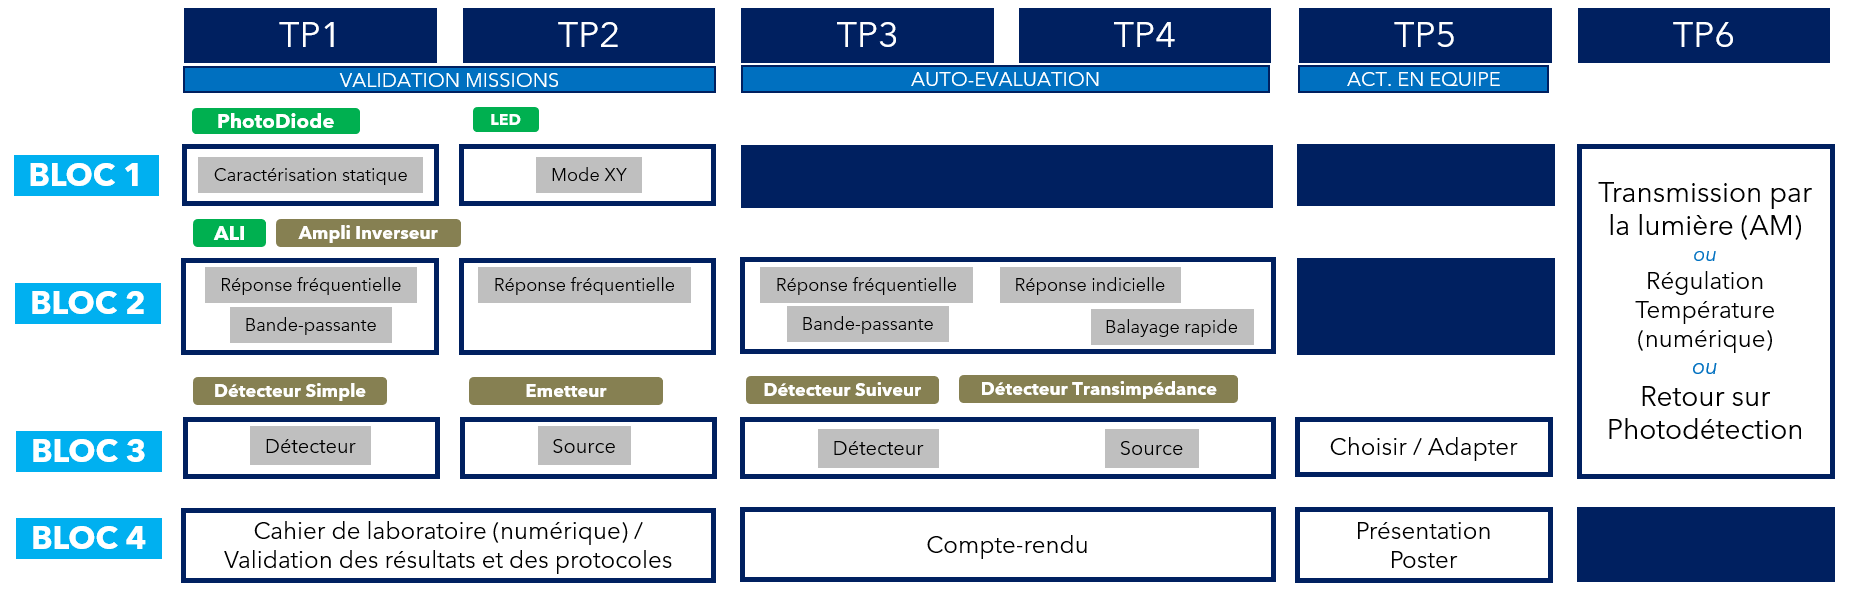
\includegraphics[width=\textwidth]{images/deroulement_2025.png}
\end{center}

\section{Autres ressources}

Un \textbf{feuillet annexe}, présentant succinctement l'\textbf{ensemble des instruments}, est disponible sur chacune des paillasses.

Un \textbf{document annexe} contient des ressources nécessaires pour les TP : documents constructeurs, aide de cours, protocoles d'utilisation du matériel...

\medskip

\textit{L'ensemble de ces documents est également disponible sur le site du LEnsE.}

\newpage

\section{Acquis d'Apprentissage Visés - AAV}

Plus spécifiquement pour chacun des blocs suivants, les étudiant$\cdot$es seront capables de :

\subsection{Bloc 1 - caractériser un dipôle électronique (linéaire ou non-linéaire) statiquement et en déduire ses zones de fonctionnement}

\begin{description}
	\item[\colorbox{violet_iogs!70}{\textcolor{white}{B 1.1}}] Lister les \textbf{grandeurs} et les \textbf{paramètres d'intérêt} du composant à partir d'une documentation technique fournie
	\item[\colorbox{violet_iogs!70}{\textcolor{white}{B 1.2}}] Choisir les \textbf{paramètres des instruments de mesures} et des composants de protection
	\item[\colorbox{violet_iogs!70}{\textcolor{white}{B 1.3}}] Tracer la \textbf{caractéristique statique} à l'aide :
	\begin{itemize}
		\item d'un multimètre
		\item d'un oscilloscope en mode XY
	\end{itemize}
	\item[\colorbox{violet_iogs!70}{\textcolor{white}{B 1.4}}] Décrire le fonctionnement d'un montage simple à diodes
\end{description}

\subsection{Bloc 2 - caractériser un système linéaire dans les domaines temporel et fréquentiel}

\begin{description}
	\item[\colorbox{violet_iogs!70}{\textcolor{white}{B 2.1}}] Donner l'expression de la \textbf{réponse en fréquence} attendue à partir du schéma électrique d'un circuit passif ou contenant des ALI
	\item[\colorbox{violet_iogs!70}{\textcolor{white}{B 2.2}}] Tracer l'allure de la \textbf{réponse en fréquence} d'un circuit sur l'écran d'un oscilloscope par une méthode de balayage en fréquence
	\item[\colorbox{violet_iogs!70}{\textcolor{white}{B 2.3}}] Mesurer le \textbf{diagramme de Bode} en amplitude  d'un circuit linéaire point par point à l'aide :
	\begin{itemize}
		\item d'un oscilloscope
		\item d'un dB mètre
	\end{itemize}
	\item[\colorbox{violet_iogs!70}{\textcolor{white}{B 2.4}}] Mesurer un \textbf{déphasage}
	\item[\colorbox{violet_iogs!70}{\textcolor{white}{B 2.5}}] Définir et mesurer la \textbf{réponse indicielle} et/ou la \textbf{réponse impulsionnelle} d'un circuit
	\item[\colorbox{violet_iogs!70}{\textcolor{white}{B 2.6}}] Proposer un \textbf{modèle mathématique} des caractéristiques d'un circuit à partir de relevés de mesure de la réponse en fréquence et/ou de la réponse indicielle
\end{description}

\subsection{Bloc 3 - mettre en \oe{}uvre des montages de photodétection et de comparer leurs performances fréquentielles et temporelles}

\begin{description}
	\item[\colorbox{violet_iogs!70}{\textcolor{white}{B 3.1}}] Réaliser un circuit contenant une source à LED
	\item[\colorbox{violet_iogs!70}{\textcolor{white}{B 3.2}}] Caractériser un \textbf{circuit de photodétection} (simple, suiveur, transimpédance, transimpédance avec filtrage)
	\item[\colorbox{violet_iogs!70}{\textcolor{white}{B 3.3}}] Choisir et adapter les \textbf{éléments d'un circuit de photodétection} en fonction d'une application donnée
\end{description}

\subsection{Bloc 4 - documenter un travail scientifique/technique}

\begin{description}
	\item[\colorbox{violet_iogs!70}{\textcolor{white}{B 4.1}}] Documenter un cahier de laboratoire numérique partagé incluant les différents protocoles réalisés, les résultats analysés et leurs analyses
	\item[\colorbox{violet_iogs!70}{\textcolor{white}{B 4.2}}] Ecrire un compte-rendu d'une expérience scientifique
	\item[\colorbox{violet_iogs!70}{\textcolor{white}{B 4.3}}] Produire un document de communication scientifique à partir d'une expérience (en équipe)
\end{description}


\newpage


\begin{minipage}[c]{.25\linewidth}
	
\includegraphics[width=5cm]{images/LEnsE_IOGS.jpg}
\end{minipage} \hfill
\begin{minipage}[c]{.4\linewidth}

\begin{center}
\vspace{0.3cm}
{\Large \textsc{Opto-Électronique}}

\medskip

5N-027-SCI \qquad \textbf{\Large TP - Sujet}

\end{center}
\end{minipage}\hfill

\vspace{0.5cm}

\noindent \rule{\linewidth}{1pt}

{\noindent\Large  \rule[-7pt]{0pt}{30pt}
 \textbf{Travail à réaliser au cours des séances}}

\noindent \rule{\linewidth}{1pt}


\section{Livrables et cahier de laboratoire numérique}

Au cours des différentes séances, vous serez amenés à \textbf{réaliser des expériences} afin de répondre à la problématique posée par les missions proposées. 

\medskip

Dans le cadre de ces expériences, vous devrez :

\begin{enumerate}
	\item vous \textbf{approprier} la problématique
	\item proposer ou justifier un \textbf{protocole expérimental}
	\item \textbf{câbler} un circuit et le \textbf{rendre opérationnel}
	\item exécuter les protocoles expérimentaux
	\item \textbf{collecter des résultats} et les présenter de manière pertinente
	\item justifier ou proposer un \textbf{modèle mathématique}
	\item expliquer la \textbf{cohérence} entre les résultats et la problématique traitée

\end{enumerate}

\bigskip


\noindent \rule{\linewidth}{1pt}

{\large
Vous devrez \textbf{garder une trace} de l'ensemble des ces étapes dans un \textbf{cahier de laboratoire} sous forme \textbf{numérique} et \textbf{partagé} par les membres du binôme.
}

\noindent \rule{\linewidth}{1pt}

\section{Démarche scientifique}

En partant d'un \textbf{montage simple}, nous allons suivre une démarche scientifique pour \textbf{caractériser ce montage}, \textbf{en déduire son modèle mathématique} puis l'\textbf{améliorer} pour obtenir des montages aux performances dynamiques (fréquentielles ici) maitrisées.

\medskip

Pour cela, vous serez amenés à \textbf{utiliser et mettre en place des protocoles expérimentaux}, mettant en \oe{}uvre de l'instrumentation scientifique. Les \textbf{résultats obtenus} seront alors \textbf{à comparer au modèle mathématique}.

\medskip

Tout au long des séances, vous serez alors amené à \textbf{modifier le modèle} associé à chaque montage afin de prendre en compte les observations faites sur les résultats. Cela entrainera une amélioration du montage pour \textbf{améliorer les performances} et ainsi proposer un nouveau modèle puis de nouveaux essais pour le valider. Et ainsi de suite.

\newpage
\section{Approche par compétences et livrables}

Ce module d'enseignement s'inscrit dans le \textbf{déploiement de l'approche par compétences} à l'IOGS (\href{https://tinyurl.com/APC-IOGS}{APC à l'IOGS}). Dans le cadre de ce module, les compétences suivantes seront particulièrement évaluées, au niveau 1, dans le cadre de diverses activités au cours des séances :

\begin{description}
	\item[\textbf{C3}] Réaliser et développer une solution technologique
	\item[C4] Valider une solution technologique
	\item[C5] Extraire et interpréter des informations et des données
\end{description}

\textit{La description des compétences est fournie en annexe pour chacune des 3 compétences.}


\subsection{Validation de missions - séances 1 et 2}

Vous devrez faire valider, en binôme, auprès d'un$\cdot$e encadrant$\cdot$e :

\begin{itemize}
	\item une \textbf{caractéristique statique} (photodiode)
	\item une \textbf{réponse fréquentielle} (détecteur simple) incluant une \textbf{mesure de bande-passante} et de la \textbf{phase} associée
\end{itemize}

Vous devrez présenter l'ensemble des livrables attendus pour justifier de la validité de vos résultats : protocoles, résultats, analyse et comparaison au modèle théorique. %Lors de cette validation, il peut vous être demandé de faire à nouveau une des mesures présentées.


\subsection{Compte-rendu - séance 4}

Un \textbf{compte-rendu} par binôme est à remettre en fin de séance 4.

\textit{Ce compte-rendu devra porter sur l'un des 3 montages réalisés au cours des séances 3 ou 4.}

Ce document synthétique et riche de preuves (basées sur vos résultats expérimentaux) a pour objectif de revendiquer le fait que vous êtes \textbf{capable de réaliser et de caractériser un système linéaire dans les domaines temporel et fréquentiel}.

\textit{Une grille d'auto-évaluation, identique à celle permettant d'évaluer les comptes-rendus de TP d'Optique, est fournie à la fin de ce document.}

\subsubsection{Paragraphe sur l'impact sociétal et environnemental}

Votre compte-rendu devra également \textbf{intégrer un paragraphe autour de l'impact sociétal et environnemental} de l'utilisation des 3 composants utilisés : LED, photodiode et amplificateur opérationnel/linéaire intégré.

Ce paragraphe devra faire clairement ressortir les \textbf{précautions à prendre} pour la mise en \oe{}uvre de chacun de ces composants (grandeurs électriques limitantes), ainsi que leur \textbf{prix} et leur \textbf{impact carbone}.


Quelques ressources :

\begin{itemize}
	\item \href{https://base-empreinte.ademe.fr/}{https://base-empreinte.ademe.fr/}
	\item \href{https://www.openlca.org/}{https://www.openlca.org/}
	\item \href{https://www.glimpact.com/european-global-impact-score}{https://www.glimpact.com/european-global-impact-score}
\end{itemize}

\subsection{Autres activités - séances 3 à 5}

Un \textbf{test individuel} est prévu en séance 3 ou 4 (voir planning fourni lors de la séance 2) et un \textbf{atelier par équipe} en séance 5.

\textit{Pour ces activités, veuillez vous référer au site du LEnsE, dans la rubrique Année / Première Année / Opto-Electronique S5 / Modalités.}



\medskip

% Séances
\cleardoublepage
\ifodd\value{page}\else
  \hbox{}\newpage
\fi

\newpage
%\pagestyle{empty}

\begin{minipage}[c]{.25\linewidth}
	
\includegraphics[width=4cm]{images/Logo-LEnsE.png}
\end{minipage} \hfill
\begin{minipage}[c]{.4\linewidth}

\begin{center}
\vspace{0.3cm}
{\Large \textsc{Opto-Électronique}}

\medskip

5N-027-SCI \qquad \textbf{\Large TP Séance 1}

\end{center}
\end{minipage}\hfill

%%%%%%%%%%%%%%%%%%%%%%%%%%%%%%%%%%
\section{Objectif de la séance}

Lors de cette première séance, vous allez :

\begin{itemize}
	\item étudier un premier \textbf{montage de photodétection} et déterminer certaines de ses caractéristiques
	\item \textbf{caractériser statiquement le capteur} de ce montage, la photodiode
	\item \textbf{mettre en \oe{}uvre un montage d'amplification} basé sur un amplificateur linéaire intégré (ALI) et le \textbf{caractériser fréquentiellement} et \textbf{temporellement}
\end{itemize} 

\medskip

Vous allez également vous \textbf{familiariser avec l'utilisation des appareils de mesure} mis à
votre disposition au cours des séances de Travaux Pratiques d'Opto-Électronique et \textbf{mettre en \oe{}uvre des protocoles expérimentaux standards} en photonique.

%%%%%%%%%%%%%%%%%%%%%%%%%%%%%%%%%%
\section{Etude d'un montage simple de photodétection - \textit{Durée : 90 min}}

On s'intéresse au circuit de la figure~\ref{fig:schem_photo} avec $E = 5 \, V$ (tension continue), une photodiode de type \textbf{\texttt{SFH206K}} (documentation fournie dans le document annexe) et $R_{PHD} = 100 \, k\Omega$:

\begin{figure}[h!]
    \centering
\begin{circuitikz}
	\draw (0,0) to[battery2, invert] (0,3) -- (2,3);
	% fleche
	\draw (-0.5,0.3) edge[->] (-0.5,2.7);
	\node (Ein) at (-1,1.5){$E$};
	
	\draw (5,3) to[empty photodiode] (2,3);
	\draw (2,3) to[short, i = $I_{photo}$, current arrow scale=8] ++(0.5,0);

	\draw (5,3) to[R=$R_{PHD}$, *-*] (5,0) -- (0,0);
	\draw (5,0) to[short, -o] ++(1.5,0);
	\draw (5,3) to[short, -o] ++(1.5,0);
	\draw (5,0) node[ground](GND){};
	% fleche
	\draw (6.5,0.3) edge[->, green!40!black] (6.5,2.7); 
	\node[text=green!40!black] (US) at (7.1,1.5){$V_S$};

	\node (PhiE) at (3,2){$\Phi_e$};	
	
\end{circuitikz}
    \caption{Schéma du circuit de photodétection simple}
    \label{fig:schem_photo}
\end{figure}

On souhaite pouvoir remplir le tableau suivant (à reproduire dans votre cahier de laboratoire) :

\medskip

\begin{center}
\begin{tabular}{|c|c|c|c|c|}
  \hline
  Grandeur & Unité & Flux ambiant & Obscurité & Lampe de bureau \\
  \hline
  Intensité lumineuse $\Phi_e$ &  &  &  &  \\
  \hline
  Tension $V_S$ &  &  &  &  \\
  \hline
  Courant $I_{photo}$ &  &  &  &  \\
  \hline
\end{tabular}
\end{center}

\Quest Proposer des protocoles (avec les schémas associés incluant les appareils de mesure) pour remplir ce tableau.

\Quest Quel est le lien entre la tension $V_S$ et le flux lumineux mesuré $\Phi_e$ ?

\medskip

\Manip Câbler le montage ci-dessus, en incluant les instruments de mesure adéquats et relever les informations nécessaires pour le tableau précédent.

\Quest Chercher dans la documentation technique de la photodiode la valeur de la \textbf{sensibilité spectrale} et comparer le courant mesuré au courant théorique. Que pouvez-vous conclure ?

\Manip Visualiser la tension aux bornes de $R_{PHD}$ à l'aide d'un oscilloscope et comparer le signal observé au signal attendu. 


\clearpage
%%%%%%%%%%%%%%%%%%%%%%%%%%%%%%%%%%
%%%%%%%%%%%%%%%%%%%%%%%%%%%%%%%%%%
%%%%%%%%%%%%%%%%%%%%%%%%%%%%%%%%%%
\section{Etude statique d'une photodiode - \textit{Durée : 60 min}}

Le système de photodétection précédent inclus un \textbf{capteur particulier}, une photodiode, que nous allons à présent chercher à \textbf{caractériser statiquement}, c'est à dire de \textbf{tracer expérimentalement la loi mathématique} qui lie le courant traversant le dipôle et la différence de potentiel à ses bornes.


%%%%%%%%%%%%%%%%%%%%%%%%%%%%%%%%%%
\subsection{Ressources}

\begin{itemize}
	\item Fiche : Diode / LED / Photodiode
	\item Fiche : Photodétection
	\item Protocole : Caractéristique statique d'un dipôle / Caractéristique Manuelle
\end{itemize}


\subsection{Photodiode \texttt{SFH206K}}

On utilisera une photodiode de type \textbf{\texttt{SFH206K}} (une partie de la documentation est fournie en annexe).

\Quest Rechercher et relever dans la documentation technique du constructeur de la photodiode \texttt{SFH206K} les valeurs intéressantes pour la mise en \oe{}uvre pratique (électrique et optique) d'un tel composant.


\subsection{Choix des appareils et des composants}

Dans le schéma proposé dans la rubrique \textbf{Caractéristique manuelle} du tutoriel \textit{Caractéristique statique d'un dipôle}, une résistance $R_P$ est proposée comme protection en courant.

\Quest Comment choisir cette résistance et comment régler les différents appareils de mesure?

\Manip Relever la caractéristique $i=f(u)$ de cette photodiode, lorsqu'elle est plongée dans l'obscurité, pour des tensions $u$ positives ET négatives.

\Manip Relever la caractéristique $i=f(u)$ de cette photodiode, lorsqu'elle est soumise à un flux lumineux constant, pour des tensions $u$ positives ET négatives. Quelle précaution faut-il prendre lors de cette mesure ?

\Manip Déterminer les zones d'utilisation possible de ce composant. Quel modèle peut-on alors proposer pour ce capteur ? 

%%%%%%%%%%%%%%%%%%%%%%%%%%%%%%%%%%
\subsection{Validation des résultats}

\Real Préparer une présentation (3-4 min maximum) rassemblant les \textbf{schémas de mesure}, les \textbf{protocoles utilisés}, les \textbf{calculs réalisés}, les \textbf{résultats pertinents} obtenus ainsi qu'une \textbf{brève analyse} de ces derniers.

\medskip

\noindent \rule{\linewidth}{1pt}

\textbf{\Large Faire valider l'ensemble par un$\cdot$e encadrant$\cdot$e}

\medskip

Cette présentation devra clairement faire ressortir des preuves en lien avec :

\begin{itemize}
	\item les compétences \fbox{C3}, \fbox{C4} et \fbox{C5}
	\item les AAV du \fbox{bloc 1}
\end{itemize}



\clearpage
%%%%%%%%%%%%%%%%%%%%%%%%%%%%%%%%%%
%%%%%%%%%%%%%%%%%%%%%%%%%%%%%%%%%%
%%%%%%%%%%%%%%%%%%%%%%%%%%%%%%%%%%
\section{Etude fréquentielle d'un montage amplificateur - \textit{Durée : 120 min}}

On se propose d'étudier le circuit \textbf{amplificateur inverseur} dont le schéma est donné dans la figure~\ref{fig:schem_ampli} :

\begin{figure}[h!]
    \centering
\begin{circuitikz} 
	\node [op amp, fill=blue!10!white](A1) at (0,0){\texttt{AOP1}};
	\draw (A1.-) to[short] ++(-.5,0) coordinate(A) to[short] ++(0,1.5) coordinate(B) to[R=$R_2$] (B -| A1.out) to[short, -*] (A1.out);
	\draw (A1.-) to[short,-*] ++(-.5,0) coordinate(AA) to[R=$R_1$] ++(-2.5,0) coordinate(BB) to[short,-o] ++(-.5,0) coordinate(CC);
	\draw (A1.+) to[short] ++(0,-0.5) node[ground]{};
	\draw (A1.out) to[short,-o] ++(1,0) coordinate(D);
	\draw (-4.6,-1) edge[->,color={green!40!black}] (-4.6,0.3);
	\node[text={green!40!black}] (Ve) at (-5.1,-0.35){$V_e$}; 
	\draw (-4.6,-1.3)  to[open,-o] ++(0,0) node[ground](GND){};
	\draw (2.2,-1) edge[->, color={red}] (2.2,-0.3);
	\node[text={red}] (Vs) at (1.7,-0.6){$V_s$}; 
	\draw (2.2,-1.3)  to[open,-o] ++(0,0) node[ground](GND){};
	
\end{circuitikz}
    \caption{Schéma d'un circuit amplificateur inverseur}
    \label{fig:schem_ampli}
\end{figure}

Ce montage utilise un \textbf{amplificateur linéaire intégré (ALI)}. Pour ce TP, on choisira un ALI de type \textbf{\texttt{TL081}}.

\medskip

On peut montrer que la fonction de transfert théorique d'un tel montage vaut :

\[
\boxed{\frac{V_s}{V_e} = - \frac{R_2}{R_1}}
\]

\medskip

On souhaite \textbf{vérifier que cette loi reste valable} quelque soit la fréquence et l'amplitude du signal d'entrée.

\medskip

Pour cela, on souhaite pouvoir remplir le tableau suivant (à reproduire dans votre cahier de laboratoire) :

\medskip

\begin{center}
\begin{tabular}{|c|c|c|c|c|c|c|}
  \hline
  Gain (dB) & [A]mplification & $R_1$ & $R_2$ & [B]ande [P]assante & Produit [A].[BP] & $\Delta{}T_{95\%}$\\
  \hline
  $12$ &  &  &  & & & \\
  \hline
  $32$ &  &  &  & & & \\
  \hline
\end{tabular}
\end{center}

où l'amplification correspond à $\frac{V_s}{V_e}$, $R_1$ et $R_2$ les valeurs des résistances choisies, la bande-passante à $-3\operatorname{dB}$ et $\Delta{}T_{95\%}$ est le temps de réponse à 95\%.



\subsection{Ressources}

\begin{itemize}
	\item Fiche : Amplificateur Linéaire Intégré
	\item Fiche : Amplificateur Linéaire Intégré / Modèle
	\item Fiche : Régime Harmonique
	\item Fiche : Filtrage / Analyse Harmonique / Ordre 1
	\item Protocole : Réponse en fréquence d'un système linéaire / Procédure "classique"
	\item Protocole : Réponse indicielle d'un système linéaire
\end{itemize}


\clearpage
\subsection{Alimentation symétrique}
Certains composants, notamment les amplificateurs linéaires intégrés, sont capables de traiter des différences de potentiel positives et négatives. Pour cela, il est nécessaire de les alimenter de manière symétrique, c'est-à-dire, avec deux sources de tension fournissant des tensions opposées, souvent notées \texttt{+VCC}, pour l'alimentation positive, et \texttt{-VCC}, pour l'alimentation négative. 

\Quest A partir de la documentation technique, noter le câblage du composant \textbf{\texttt{TL081}} et les tensions d'alimentation maximales. 

\Manip Réaliser une \textbf{alimentation symétrique +10V / -10V} à partir des alimentations stabilisées disponibles et mettre en place un système de contrôle de ces tensions.

\Quest Quelles précautions faudra-t-il prendre sur la tension d'entrée de ce montage ?

%%%%%%%%%%%%%%%%%%%%%%%%%%%%%%%%%%
\subsection{Réponse en fréquence}

\Quest Quelles valeurs de résistances choisir pour obtenir un gain de $12~\operatorname{dB}$ ? \textit{La somme des résistances doit être comprise entre $10\operatorname{k\Omega}$ et $50\operatorname{k\Omega}$.}

\Manip Réaliser le montage précédent et alimenter le avec l'alimentation symétrique réalisée.

\Manip Tracer le \textbf{diagramme de Bode en gain} de ce système pour des fréquences allant de $100~\operatorname{Hz}$ à $1~\operatorname{MHz}$, à l'aide de mesure réalisée à l'oscilloscope. 

\Quest Quelle était la réponse en fréquence attendue théoriquement ? 

\Manip Mesurer la bande-passante à $-3\operatorname{dB}$ de ce montage.

%%%%%%%%%%%%%%%%%%%%%%%%%%%%%%%%%%
\noindent \rule{\linewidth}{1pt}

\Manip Modifier la résistance $R_1$ pour obtenir un gain de $32~\operatorname{dB}$.

\Manip Tracer le \textbf{diagramme de Bode en gain} de ce système pour des fréquences allant de $100~\operatorname{Hz}$ à $1~\operatorname{MHz}$, à l'aide de mesure réalisée à l'oscilloscope. 

\Manip Mesurer la bande-passante à $-3\operatorname{dB}$ de ce nouveau montage.

\Quest Préciser alors le modèle à utiliser pour ce montage. 


%%%%%%%%%%%%%%%%%%%%%%%%%%%%%%%%%%
\subsection{Réponse indicielle}

\Manip Pour les deux montages précédents, visualiser la réponse indicielle.

\Manip Mesurer le temps de réponse à 95\%.

\Quest Quel est le lien entre ce temps et la bande-passante mesurée dans la partie précédente ?


%%%%%%%%%%%%%%%%%%%%%%%%%%%%%%%%%%
%%%%%%%%%%%%%%%%%%%%%%%%%%%%%%%%%%
\subsection{Cahier de laboratoire / Check-List}

\begin{itemize}[label=$\square$]
	\item tableau comparatif rempli
	\item protocoles utilisés (avec schéma de câblage, paramètres des instruments de mesure et étapes expérimentales)
	\item diagrammes de Bode légendés
	\item captures d'écran d'oscilloscope des réponses indicielles
	\item analyse des résultats
	\item modélisation du système
\end{itemize}




%%%%%%%%%%%%%%%%%%%%%%%%%%%%%%%%%%%%%%%%%%%%%%%%%%%%%%%%%%%%%%%%%%%%%%%%%%%%%%%%%%%%%

\cleardoublepage
\ifodd\value{page}\else
  \hbox{}\newpage
\fi
\newpage
%\pagestyle{empty}

\begin{minipage}[c]{.25\linewidth}
	
\includegraphics[width=4cm]{images/LEnsE_IOGS.jpg}
\end{minipage} \hfill
\begin{minipage}[c]{.4\linewidth}

\begin{center}
\vspace{0.3cm}
{\Large \textsc{Opto-Électronique}}

\medskip

5N-027-SCI \qquad \textbf{\Large TP Séance 2}

\end{center}
\end{minipage}\hfill

%%%%%%%%%%%%%%%%%%%%%%%%%%%%%%%%%%
\section{Objectif de la séance}

Lors de cette seconde séance, vous allez :

\begin{itemize}
	\item mettre en place un \textbf{banc de caractérisation} d'un montage de photodétection
	\begin{itemize}
		\item \textbf{caractériser statiquement une LED}	
		\item réaliser un \textbf{émetteur de flux lumineux} basé sur une source à LED
	\end{itemize} 
	
	\item mettre en \oe{}uvre un \textbf{montage simple de photodétection} et le \textbf{caractériser fréquentiellement} et \textbf{temporellement}
\end{itemize} 


%%%%%%%%%%%%%%%%%%%%%%%%%%%%%%%%%%
\subsection{Premier modèle du montage de photodétection}

Les premiers résultats obtenus lors de la précédente séance autour du montage simple de photodétection ont permis de conclure que ce type de montage permettait d'\textbf{obtenir une tension proportionnelle au flux lumineux}.

\medskip

On peut montrer que la fonction de transfert théorique d'un tel montage vaut :

\[
\boxed{V_s = R_{PHD} \cdot I_{photo} = R_{PHD} \cdot k \cdot \Phi_{e}}
\]

où $k$ est la sensibilité de la photodiode et $\Phi_e$ le flux lumineux à mesurer.

%%%%%%%%%%%%%%%%%%%%%%%%%%%%%%%%%%
\subsection{Validité du modèle}

On souhaite \textbf{vérifier que cette loi reste valable} quelque soit la fréquence et l'amplitude du flux lumineux d'entrée.

\medskip

Pour cela, on souhaite pouvoir remplir le tableau suivant (à reproduire dans votre cahier de laboratoire) et \textbf{mesurer la réponse en fréquence de ce montage} :

\medskip

\begin{center}
\begin{tabular}{|c|c|c|c|c|c|}
  \hline
  $R_{PHD}$ & $|V_s|_{MAX}$ & [B]ande [P]assante & [BP]/$R_{PHD}$ \\
  \hline
  $10\operatorname{k\Omega}$ & & & \\
  \hline
  $100\operatorname{k\Omega}$ & & & \\
  \hline
  $1\operatorname{M\Omega}$ & & & \\
  \hline
\end{tabular}
\end{center}

où $|V_s|_{MAX}$ est l'amplitude maximale du signal de sortie, [BP] est la bande-passante à $-3\operatorname{dB}$ du système et [BP]/$R_{PHD}$ le rapport de la bande-passante sur la valeur de la résistance $R_{PHD}$.

\bigskip

%%%%%%%%%%%%%%%%%%%%%%%%%%%%%%%%%%
\subsection{Nécessité d'une source lumineuse paramètrable}

Afin de pouvoir étudier le montage de photodétection pour différentes fréquences, il est \textbf{indispensable} d'avoir à disposition \textbf{une source lumineuse dont la fréquence du flux lumineux est modifiable}.


\clearpage
%%%%%%%%%%%%%%%%%%%%%%%%%%%%%%%%%%
%%%%%%%%%%%%%%%%%%%%%%%%%%%%%%%%%%
%%%%%%%%%%%%%%%%%%%%%%%%%%%%%%%%%%
\section{Etude statique d'une LED - \textit{Durée : 60 min}}

Nous allons chercher à \textbf{caractériser statiquement} une source lumineuse de type \textbf{LED}, c'est à dire \textbf{tracer expérimentalement la loi mathématique} qui lie le courant traversant le dipôle et la différence de potentiel à ses bornes.


%%%%%%%%%%%%%%%%%%%%%%%%%%%%%%%%%%
\subsection{Ressources}

\begin{itemize}
	\item Fiche : Diode / LED / Photodiode
	\item Protocole : Caractéristique statique d'un dipôle / Caractéristique Manuelle
\end{itemize}

%%%%%%%%%%%%%%%%%%%%%%%%%%%%%%%%%%
\subsection{LED Rouge}

On utilisera une LED Rouge de type \textbf{\texttt{Kingbright L-1503ID}} (une partie de la documentation est fournie en annexe).

\Quest Rechercher et relever, dans la documentation technique du constructeur de la LED Rouge, les valeurs intéressantes pour la mise en \oe{}uvre pratique (électrique et optique) d'un tel composant.


\subsection{Choix des appareils et des composants}

Dans le schéma proposé dans la rubrique \textbf{Caractéristique manuelle} du tutoriel \textit{Caractéristique statique d'un dipôle}, une résistance $R_P$ est proposée comme protection en courant.

\Quest Comment choisir cette résistance et comment régler les différents appareils de mesure?

\Manip Relever la caractéristique $i=f(u)$ de cette LED pour des tensions $u$ positives ET négatives. 

\Manip Déterminer les zones d'utilisation possible de ce composant. 

\medskip

%%%%%%%%%%%%%%%%%%%%%%%%%%%%%%%%%%
\subsection{Cahier de laboratoire / Check-List}

\begin{itemize}[label=$\square$]
	\item protocoles utilisés (avec schéma de câblage, paramètres des instruments de mesure et étapes expérimentales)
	\item courbe de la caractéristique statique
	\item analyse de la courbe
\end{itemize}

%%%%%%%%%%%%%%%%%%%%%%%%%%%%%%%%%%
%%%%%%%%%%%%%%%%%%%%%%%%%%%%%%%%%%
\clearpage
\section{Réalisation d'un émetteur lumineux - \textit{Durée : 60 min}}

Afin de pouvoir caractériser en fréquence le montage de photodétection, nous allons avoir besoin d'un émetteur lumineux dont il est possible de \textbf{contrôler la fréquence du flux lumineux émis} (voir circuit sur la figure~\ref{fig:schem_emit_trans}).

\begin{figure}[h!]
    \centering
\begin{circuitikz}
	\draw (-2,0) to[short, o-*] (-1, 0) -- (0, 0) to[R=$R_{LED}$] (0, 2);
	\draw (-2, 4.5) to[short, o-] (0, 4.5) to[led, l_=$LED$] (0, 2);
	\draw (-1,0) node[ground](GND){};
	\draw (-2,0.3) edge[->, red!40!black] (-2,4.2);
	\node[text=red!40!black] (Vin) at (-2.5,2.25){$V_e$};
	
	\draw[->, thick, blue!40!black, decorate, decoration={snake, amplitude=1mm, segment length=4mm}] (0.8,3.25) -- (2.2,3.25);
	\node[text=blue!40!black] (Phi) at (1.5,4){$\Phi_e$};

	\draw (7,0) to[battery2, invert] (7,4.5) -- (3,4.5);
	% fleche
	\draw (7.5,0.3) edge[->, thick] (7.5,4.2);
	\node (Ein) at (8,2.25){$E$};
	
	\draw (3,2) to[empty photodiode, -] (3,4.5);
	\draw (3,2.8) to[short, i = $I_{photo}$, current arrow scale=8] ++(0,-0.5);

	\draw (3,2) to[R=$R_{PHD}$, *-] (3,0) to[short, -*] (4,0) -- (7,0);
	\draw (3,2) to[short, -o] ++(1.5,0);
	\draw (4,0) node[ground](GND){};
	% fleche
	\draw (4.5,0.3) edge[->, thick, green!40!black] (4.5,1.7); 
	\node[text=green!40!black] (US) at (5,1){$V_S$};
\end{circuitikz}
    \caption{Schéma du circuit émetteur (à gauche) et du circuit de photodétection simple (à droite)}
    \label{fig:schem_emit_trans}
\end{figure}

où $\Phi_e$ est le flux lumineux résultant de l'émetteur.

\medskip

On souhaite un \textbf{flux lumineux sinusoïdal} dont il est possible de contrôler la fréquence de modulation. \textit{Attention, on ne parle pas ici de la variation de la longueur d'onde de la source lumineuse mais bien de la modulation du flux lumineux en amplitude.}

\Quest Quel signal doit-on appliquer sur $V_e$ ? Quels sont les paramètres à donner à ce signal (amplitude, valeur moyenne...) pour obtenir un flux lumineux sinusoïdal ?

\Quest A quoi correspond la résistance $R_{LED}$ ? Comment vérifier que le flux est sinusoïdal (sans utiliser le montage de photodétection proposé puisqu'on ne connaît pas sa réponse en fréquence) ?

\Manip Réaliser le système d'émission et vérifier son bon fonctionnement.


%%%%%%%%%%%%%%%%%%%%%%%%%%%%%%%%%%
\subsection{Cahier de laboratoire / Check-List}

\begin{itemize}[label=$\square$]
	\item paramètres utilisés pour le générateur $V_e$
	\item protocole de vérification de la forme du flux lumineux
	\item validation du fonctionnement (capture d'écran d'oscilloscope)
\end{itemize}


%%%%%%%%%%%%%%%%%%%%%%%%%%%%%%%%%%
\subsection{Montage de photodétection - Rappel}

Dans le circuit précédent, la partie de droite correspond au montage de photodétection que nous allons par la suite chercher à caractériser.

\Quest A quoi sert la tension $E$ ? De quelle nature doit-elle être ?

\Quest Quelle fonction de transfert cherche-t-on à caractériser sur ce montage de photodétection ? 

\Quest A-t-on accès directement à la valeur du flux lumineux $\Phi_e$ ? De quoi dépend le flux lumineux reçu par la photodiode (en lien avec celui émis par la LED) ? Quelles seront alors les précautions à prendre lors des prochaines mesures ?



\clearpage
%%%%%%%%%%%%%%%%%%%%%%%%%%%%%%%%%%
%%%%%%%%%%%%%%%%%%%%%%%%%%%%%%%%%%
%%%%%%%%%%%%%%%%%%%%%%%%%%%%%%%%%%
\section{Réponse en fréquence du montage - \textit{Durée : 120 min}}

On souhaite à présent \textbf{vérifier la validité du modèle proposé initialement} pour le montage simple de photodétection pour des flux lumineux modulés à différentes fréquences.

Pour cela, on placera le système émetteur devant le montage de photodétection à caractériser (voir schéma de la section précédente).

\subsection{Ressources}

\begin{itemize}
	\item Fiche : Photodétection
	\item Fiche : Filtrage / Analyse Harmonique / Ordre 1
	\item Protocole : Réponse en fréquence d'un système linéaire / Procédure "classique"
	\item Protocole : Mesure de bande-passante
	\item Protocole : Réponse indicielle d'un système linéaire
\end{itemize}



%%%%%%%%%%%%%%%%%%%%%%%%%%%%%%%%%%
\subsection{Réponse en fréquence}

\Manip Placer le montage émetteur face au montage de photodétection (la LED en face de la partie sensible de la photodiode). Utiliser une résistance $R_{PHD} = 100\operatorname{k\Omega}$.

\Manip Tracer le \textbf{diagramme de Bode en gain} de ce système pour des fréquences allant de $100~\operatorname{Hz}$ à $1~\operatorname{MHz}$, à l'aide de mesure réalisée à l'oscilloscope.

\Quest Quelle était la réponse en fréquence attendue théoriquement ? 

\Manip Mesurer la bande-passante à $-3\operatorname{dB}$ de ce montage.

\medskip

\Manip Refaire le tracé du diagramme de Bode et la mesure de la bande-passante pour des résistances $R_{PHD} = 10\operatorname{k\Omega}$ et $R_{PHD} = 1\operatorname{M\Omega}$

\Quest Conclure sur le modèle à utiliser pour ce montage. 



%%%%%%%%%%%%%%%%%%%%%%%%%%%%%%%%%%
\subsection{Validation des résultats}

\Real Préparer une présentation (3-4 min maximum) rassemblant les \textbf{schémas de mesure}, les \textbf{protocoles utilisés}, les \textbf{calculs réalisés}, les \textbf{résultats pertinents} obtenus ainsi qu'une \textbf{brève analyse} de ces derniers.

\medskip

\noindent \rule{\linewidth}{1pt}

\textbf{\Large Faire valider l'ensemble par un$\cdot$e encadrant$\cdot$e}

\medskip

Cette présentation devra clairement faire ressortir des preuves en lien avec :

\begin{itemize}
	\item les compétences \fbox{C3}, \fbox{C4} et \fbox{C5}
	\item les AAV du \fbox{bloc 2}
\end{itemize}



%%%%%%%%%%%%%%%%%%%%%%%%%%%%%%%%%%%%%%%%%%%%%%%%%%%%%%%%%%%%%%%%%%%%%%%%%%%%%%%%%%%%%


\cleardoublepage
\ifodd\value{page}\else
  \hbox{}\newpage
\fi
\newpage
%\pagestyle{empty}

\begin{minipage}[c]{.25\linewidth}
	
\includegraphics[width=4cm]{images/LEnsE_IOGS.jpg}
\end{minipage} \hfill
\begin{minipage}[c]{.4\linewidth}

\begin{center}
\vspace{0.3cm}
{\Large \textsc{Opto-Électronique}}

\medskip

5N-027-SCI \qquad \textbf{\Large TP Séances 3/4}

\end{center}
\end{minipage}\hfill

%%%%%%%%%%%%%%%%%%%%%%%%%%%%%%%%%%
\section{Auto-évaluation - \textit{Durée : 120 min}}

Au cours de l'une des séances 3 ou 4, vous aurez à réaliser une \textbf{auto-évaluation pratique} selon le planning transmis par les responsables du module.

Cette auto-évaluation portera sur la \textbf{caractérisation statique d'un  composant} et la \textbf{caractérisation en fréquence d'un système}.

\medskip

\textit{Les modalités du module d'Opto-Electronique sont données sur les site Internet du LEnsE.}

%%%%%%%%%%%%%%%%%%%%%%%%%%%%%%%%%%
\section{Objectif des séances}

Lors de ces séances, vous allez :

\begin{itemize}
	\item utiliser le \textbf{banc de caractérisation} mis en place précédemment pour :
	\begin{itemize}
		\item  \textbf{caractériser fréquentiellement} et \textbf{temporellement} différents montages de photodétection
		\item comparer les performances de chacun de ces montages
	\end{itemize} 
\end{itemize} 




%%%%%%%%%%%%%%%%%%%%%%%%%%%%%%%%%%
\section{Éléments à prendre en considération pour la modélisation}

Afin d'expliquer le phénomène observé précédemment, il est possible d'affiner le modèle utilisé pour l'étude du montage précédent en prenant en compte les éléments "perturbateurs".

La figure~\ref{fig:schem_model} présente le schéma du modèle plus complet du circuit étudié précédemment.

\begin{figure}[h!]
    \centering
\begin{circuitikz}
	% blocs
	\fill[green,fill opacity=.1] (-0.4,-0.2) rectangle (0.5,5.2);
	\fill[blue,fill opacity=.1] (4.8,2.2) rectangle (10.6,-0.2);	
	\fill[orange,fill opacity=.1] (1.5,5.2) rectangle (5.1,2.3);
	% legende blocs
	%\fill[green,fill opacity=.1] (9,5.5) rectangle (11,4.7);
	%\node (pol) at (10,5.1){Polarisation};
	%\fill[orange,fill opacity=.1] (9,4.5) rectangle (11,3.7);
	%\node (pol) at (10,4.1){Photodiode};	
	%\fill[blue,fill opacity=.1] (9,3.5) rectangle (11,2.7);
	%\node (pol) at (10,3.1){Affichage};	
	% circuit
	\draw (-0.5,0.3) edge[->] (-0.5,4.7); \node (Ein) at (-1,2.5){$E$};
	\draw (0,0) to[battery2, invert] (0,5) -- (2,5) to[I, *-*] (2,2.5) -- (2,2) to[R=$R_{PHD}$, *-*] (2,0) -- (0,0);
	\draw (2,3.3) to[short, i = $ I_{photo}$, current arrow scale=10] ++(0,-0.5);
	\draw (2,5) -- (3.5,5) to[C=$C_{PHD}$] (3.5,2.5) -- (2,2.5);
	\draw (1.3,2.8) edge[->] (1.3,4.7); 	\node (Ud) at (0.7,3.5){$u_d$};
		
	\draw (3.5,0.3) edge[->, green!40!black] (3.5,1.7); \node[text=green!40!black] (US) at (4,1){$V_S$};
	
	\draw (2,2) -- (5.5,2) to[C=$C_{cab}$, *-*] (5.5,0) -- (2,0);
	\draw (5.5,2) -- (7.5,2) to[C=$C_{osc}$, *-*] (7.5,0) -- (5.5,0);
	\draw (7.5,2) -- (9.5,2) to[R=$R_{osc}$] (9.5,0) -- (7.5,0);

\end{circuitikz}
    \caption{Schéma du modèle équivalent du circuit de photodétection simple, incluant le système de mesure (oscilloscope et câble coaxial)}
    \label{fig:schem_model}
\end{figure}


\Quest A quoi correspondent les différents éléments présents ?

\Quest A partir des mesures réalisées précédemment, comment remonter aux valeurs du modèle précédent ? Donner les valeurs des différents éléments qu'il est possible de calculer.



\clearpage
%%%%%%%%%%%%%%%%%%%%%%%%%%%%%%%%%%
\section{Optimisation des performances / Démarche}

Dans les \textbf{3 étapes} décrites par la suite, qui correspondent à une amélioration du montage de photodétection, vous devrez être en mesure de pouvoir \textbf{comparer les grandeurs caractéristiques de ces montages}.

\subsection{Comparaison des caractéristiques fréquentielles et temporelles}

Vous devrez, en particulier, vous intéresser, pour chacun de ces systèmes, à :

\begin{itemize}
	\item la \textbf{réponse en fréquence} en faisant varier la résistance $R_{PHD}$ pour voir l'influence de ce paramètre sur leur \textbf{bande-passante} et la fréquence de résonance lorsqu'il y a lieu
	\item la \textbf{réponse à un échelon} (indicielle) en faisant varier la résistance $R_{PHD}$ pour voir l'influence de ce paramètre sur le \textbf{temps de réaction} du système
\end{itemize} 

\medskip

Pour cela, on souhaite pouvoir remplir le tableau suivant (à reproduire dans votre cahier de laboratoire) et \textbf{mesurer la réponse en fréquence des quatre circuits} proposés (incluant le circuit simple de photodétection) :

\medskip

\begin{center}
\begin{tabular}{|c|c|c|c|c|c|}
  \hline
  $R_{PHD}$ & $|V_s|_{MAX}$ & [B]ande [P]assante & [BP]/$R_{PHD}$ & Temps de réponse\\
  \hline
  $10\operatorname{k\Omega}$ & & & & \\
  \hline
  $100\operatorname{k\Omega}$ & & & & \\
  \hline
  $1\operatorname{M\Omega}$ & & & & \\
  \hline
\end{tabular}
\end{center}

où $|V_s|_{MAX}$ est l'amplitude maximale du signal de sortie, [BP] est la bande-passante à $-3\operatorname{dB}$ du système, [BP]/$R_{PHD}$ le rapport de la bande-passante sur la valeur de la résistance $R_{PHD}$ et le temps de réponse à 95\% du système.

\bigskip

\subsection{Etape 0 / Circuit simple de photodétection}

\textbf{Hypothèse} : une photodiode, dans sa zone de fonctionnement en capteur, produit un courant proportionnel au flux lumineux qu'elle reçoit

\textbf{Réalisation} : mise en série de la photodiode avec une résistance pour convertir le courant en une différence de potentiel mesurable et visualisable en fonction du temps

\newpage
\subsection{Etape 1 / Suiveur}

\textbf{Hypothèse} : l'ajout d'un suiveur permet d'isoler le circuit de mesure (oscilloscope et câbles) de la partie photodétection

\textbf{Réalisation} : mise en place d'un montage suiveur en cascade avec le montage simple de photodétection

\textbf{Résultats attendus} : augmentation de la bande-passante du système de photodétection (dépendance à $R_{PHD}$)



\subsection{Etape 2 / Transimpédance}


\textbf{Hypothèse} : la mise en place d'un montage transimpédance permet d'isoler la photodiode du circuit de mesure (oscilloscope et câbles) et ainsi imposer un potentiel constant à ses bornes (limitant ainsi l'impact de la capacité intrinsèque de la photodiode)

\textbf{Réalisation} : mise en place du montage transimpédance

\textbf{Résultats attendus} : augmentation de la bande-passante du système de photodétection (dépendance à $R_{PHD}$) mais apparition d'un modèle du second ordre

\textbf{Modélisation} : modélisation d'un système du second ordre (rebouclage d'un ALI avec un montage du premier ordre)

\subsection{Etape 3 / Transimpédance amélioré}

\textbf{Hypothèse} : l'ajout d'une capacité dans le montage transimpédance permet de contrôler parfaitement la bande-passante et de supprimer la résonance du montage précédent

\textbf{Réalisation} : capacité en parallèle de la résistance de contre-réaction du montage

\textbf{Résultats attendus} : légère dégradation de bande-passante du système de photodétection (dépendance à $R_{PHD}$) mais suppression de la résonance


\clearpage
%%%%%%%%%%%%%%%%%%%%%%%%%%%%%%%%%%
\section{Etape 1 / Suiveur - \textit{Durée : 120 min}}

On se propose d'\textbf{améliorer les performances dynamiques} du montage précédent en ajoutant un \textbf{montage suiveur} (basé sur un amplificateur linéaire intégré) entre le montage simple et les éléments de mesure (oscilloscope). On souhaite également \textbf{vérifier les performances dynamiques} (réponse en fréquence notamment) de ce nouveau montage et conclure sur l'intérêt de l'ajout 
d'un étage suiveur.

%%%%%%%%%%%%%%%%%%%%%%%%%%%%%%%%%%
\subsection{Ressources}

Vous pouvez utiliser les fiches résumées suivantes : 

\begin{itemize}	
	\item Protocole : Réponse en fréquence d'un système linéaire
	\item Protocole : Mesure de bande-passante
	\item Protocole : Réponse indicielle d'un système linéaire
\end{itemize}


%%%%%%%%%%%%%%%%%%%%%%%%%%%%%%%%%%
\subsection{Montage}

On se propose d'analyser le circuit de la figure~\ref{fig:schem_follow}, avec $R_{PHD} = 100\operatorname{k\Omega}$. L'amplificateur linéaire intégré sera alimenté à l'aide d'une alimentation symétrique +10V / -10V.

\medskip


\begin{figure}[h!]
    \centering
\begin{circuitikz}

	\draw (-6,0) to[short, o-*] (-5, 0) -- (-4, 0) to[R=$R_{LED}$] (-4, 2);
	\draw (-6, 4.5) to[short, o-] (-4, 4.5) to[led, l_=$LED$] (-4, 2);
	\draw (-5,0) node[ground](GND){};
	\draw (-6,0.3) edge[->, red!40!black] (-6,4.2);
	\node[text=red!40!black] (Vin) at (-6.5,2.25){$V_e$};
	
	\draw[->, thick, blue!40!black, decorate, decoration={snake, amplitude=1mm, segment length=4mm}] (-3.2,3.25) -- (-1.8,3.25);
	\node[text=blue!40!black] (Phi) at (-2.5,4){$\Phi_e$};
	
	

	\draw (0,0) to[battery2, invert] (0,4.5) -- (2,4.5);
	% fleche
	\draw (-0.5,0.3) edge[->] (-0.5,4.2);
	\node (Ein) at (-1,2.25){$E$};
	
	\draw (2,2) to[empty photodiode] (2,4.5);
	\draw (2,2.8) to[short, i = $I_{photo}$, current arrow scale=8] ++(0,-0.5);

	\draw (2,2) to[R=$R_{PHD}$, *-*] (2,0) -- (0,0);
	\draw (2,2) -- ++(2.5,0);
	\draw (1,0) node[ground](GND){};
	\draw (2,0) to[short, -o] ++(1.5,0) coordinate(VRG);
	% fleche
	\draw (3.5,0.3) edge[->, green!40!black] (3.5,1.7); \node[text=green!40!black] (UR) at (4.3,1){$V_{RPHD}$};
	\draw (3.5,0) to[short, -o] ++(0,0);
	
	\draw (4.5,2) node[op amp, fill=blue!10!white, anchor=+](A1) {\texttt{ALI1}};
	\draw (A1.-) to[short] ++(-.5,0) coordinate(A) to[short] ++(0,1.5) coordinate(B) to[short] (B -| A1.out) to[short, -*] (A1.out);
	\draw (A1.+) to[short,-o] ++(-1,0) coordinate(C);
	\draw (A1.out) to[short,-o] ++(1,0) coordinate(D);	
	\draw (VRG) -- (VRG -| A1.out) coordinate(VOUTGND);
	\draw (VOUTGND) to[short,-o] ++(1,0) coordinate(VSGND);
	
	% fleche
	\draw (VSGND) ++(0,0.3) edge[->, green!40!black] ($ (D) - (0,0.3) $); \node[text=green!40!black] (US) at ($ (VSGND)!.5!(D) + (0.5,0) $){$V_S$};	% point central entre les deux points
\end{circuitikz}
    \caption{Schéma du circuit émetteur (à gauche) et du circuit de photodétection incluant un circuit suiveur (à droite)}
    \label{fig:schem_follow}
\end{figure}

\Quest Quel est le lien entre $V_S$ et $V_{RPHD}$ ? Puis entre $V_S$ et $I_{photo}$ ? Puis entre $I_{photo}$ et le flux lumineux capté par la photodiode $\Phi_e$ ?

\Quest Quelle est la forme théorique de la réponse en fréquence de ce montage ?


%%%%%%%%%%%%%%%%%%%%%%%%%%%%%%%%%%
\subsection{Cahier de laboratoire / Check-List}

\begin{itemize}[label=$\square$]
	\item protocoles utilisés (avec schéma de câblage, paramètres des instruments de mesure et étapes expérimentales)
	\item diagrammes de Bode
	\item captures d'écran des réponses à un échelon
	\item mesures des grandeurs caractéristiques (bande-passante, temps de réponse...)
	\item analyse des différents résultats pour 3 valeurs de $R_{PHD}$ ($10\operatorname{k\Omega}$, $100\operatorname{k\Omega}$ et $1\operatorname{M\Omega}$)
	\item éléments de modélisation et lien entre les grandeurs caractéristiques et la valeur de $R_{PHD}$
\end{itemize}


\clearpage
%%%%%%%%%%%%%%%%%%%%%%%%%%%%%%%%%%
\section{Etape 2 / Transimpédance - \textit{Durée : 120 min}}

On se propose d'\textbf{étudier le montage transimpédance}, un circuit très fréquemment utilisé pour la photodétection pour ses performances dynamiques. Ce montage est basé sur un amplificateur linéaire intégré également et permet d'augmenter la bande-passante des montages vus précédemment.

On souhaite donc \textbf{vérifier les performances dynamiques} (réponse en fréquence notamment) de ce nouveau montage et conclure sur son intérêt.

%%%%%%%%%%%%%%%%%%%%%%%%%%%%%%%%%%
\subsection{Ressources}

Vous pouvez utiliser les fiches résumées suivantes (en plus de celles de l'étape précédente) : 

\begin{itemize}	
	\item Fiche : Filtrage actif / Analyse Harmonique / Ordre 2
\end{itemize}

\textit{Afin de faciliter la compréhension des phénomènes mis en jeu dans ce montage, vous pouvez vous reporter à la ressource : \textbf{Montage transimpédance : modélisation}.}

%%%%%%%%%%%%%%%%%%%%%%%%%%%%%%%%%%
\subsection{Montage}

On se propose d'analyser le circuit de la figure~\ref{fig:schem_trans}, avec $R_{PHD} = 100\operatorname{k\Omega}$. L'amplificateur linéaire intégré sera alimenté à l'aide d'une alimentation symétrique +10V / -10V.

\begin{figure}[h!]
    \centering
\begin{circuitikz} 
	\node [op amp, fill=blue!10!white](A1) at (0,0){\texttt{ALI1}};
	\draw (A1.-) to[short] ++(-.5,0) coordinate(A) to[short] ++(0,1.5) coordinate(B) to[R=$R_{PHD}$] (B -| A1.out) to[short, -*] (A1.out);
	\draw (A1.-) to[short,-*] ++(-.5,0) coordinate(AA) -- ++(-1,0) coordinate(AAA) to[empty photodiode] ++(-2,0) coordinate(BB);	
	
	\draw (AAA) to[short, i = $I_{photo}$, current arrow scale=8] ++(0.5,0);
	\draw (A1.+) to[short, -*] ++(0,-1.5) coordinate(GG) node[ground]{};
	
	\draw (A1.out) to[short,-o] ++(1,0) coordinate(D);
	
	% Ground
	\draw (GG) to[short, -o] (GG -| D);
	
	\draw (BB) to[battery2] (GG -| BB) -- (GG);
	% fleche EP
	\draw ($ (GG -| BB) + (-0.8,0.3) $) edge[->, green!40!black] ($ (BB) - (0.8,0.3) $); 
	\node[text=green!40!black] (US) at ($ (GG -| BB)!.5!(BB) - (1.5,0) $){$E_P$};
	
	% fleche VS
	\draw ($ (GG -| D) + (0,0.3) $) edge[->, green!40!black] ($ (D) - (0,0.3) $); 
	\node[text=green!40!black] (US) at ($ (GG -| D)!.5!(D) - (0.5,0) $){$V_S$};	
\end{circuitikz}    
\caption{Schéma du circuit de photodétection de type transimpédance}
    \label{fig:schem_trans}
\end{figure}

\Quest Quel est le lien entre $V_S$ et $I_{photo}$ ? Puis entre $I_{photo}$ et le flux lumineux capté par la photodiode $\Phi_e$ ?


%%%%%%%%%%%%%%%%%%%%%%%%%%%%%%%%%%
\subsection{Cahier de laboratoire / Check-List}

\begin{itemize}[label=$\square$]
	\item protocoles utilisés (avec schéma de câblage, paramètres des instruments de mesure et étapes expérimentales)
	\item diagrammes de Bode
	\item captures d'écran des réponses à un échelon
	\item mesures des grandeurs caractéristiques (bande-passante, temps de réponse, fréquence de résonance...)
	\item analyse des différents résultats pour 3 valeurs de $R_{PHD}$ ($10\operatorname{k\Omega}$, $100\operatorname{k\Omega}$ et $1\operatorname{M\Omega}$)
	\item éléments de modélisation et lien entre les grandeurs caractéristiques et la valeur de $R_{PHD}$
\end{itemize}



\clearpage
%%%%%%%%%%%%%%%%%%%%%%%%%%%%%%%%%%
\section{Etape 3 / Transimpédance amélioré - \textit{Durée : 120 min}}

On se propose de \textbf{s'affranchir d'un des défauts majeur du montage transimpédance}, sa résonance. On souhaite donc \textbf{vérifier les performances dynamiques} (réponse en fréquence notamment) de ce nouveau montage et conclure sur son intérêt.


%%%%%%%%%%%%%%%%%%%%%%%%%%%%%%%%%%
\subsection{Montage}

On se propose d'analyser le circuit de la figure~\ref{fig:schem_trans_opt}, avec $R_{PHD} = 100\operatorname{k\Omega}$. L'amplificateur linéaire intégré sera alimenté à l'aide d'une alimentation symétrique +10V / -10V.

\begin{figure}[h!]
    \centering
\begin{circuitikz} 
	\node [op amp, fill=blue!10!white](A1) at (0,0){\texttt{ALI1}};
	\draw (A1.-) to[short] ++(-.5,0) coordinate(A) to[short, -*] ++(0,1.5) coordinate(B) to[R=$R_{PHD}$] (B -| A1.out) to[short, -*] (A1.out);
	\draw (B) -- ++(0,1.5) coordinate(B2) to[C=$C_{T}$] (B2 -| A1.out) to[short,-*] (B -| A1.out);
	\draw (A1.-) to[short,-*] ++(-.5,0) coordinate(AA) -- ++(-1,0) coordinate(AAA) to[empty photodiode] ++(-2,0) coordinate(BB);	
	
	\draw (AAA) to[short, i = $I_{photo}$, current arrow scale=8] ++(0.5,0);
	\draw (A1.+) to[short, -*] ++(0,-1.5) coordinate(GG) node[ground]{};
	
	\draw (A1.out) to[short,-o] ++(1,0) coordinate(D);
	
	% Ground
	\draw (GG) to[short, -o] (GG -| D);
	
	\draw (BB) to[battery2] (GG -| BB) -- (GG);
	% fleche EP
	\draw ($ (GG -| BB) + (-0.8,0.3) $) edge[->, green!40!black] ($ (BB) - (0.8,0.3) $); 
	\node[text=green!40!black] (US) at ($ (GG -| BB)!.5!(BB) - (1.5,0) $){$E_P$};
	
	% fleche VS
	\draw ($ (GG -| D) + (0,0.3) $) edge[->, green!40!black] ($ (D) - (0,0.3) $); 
	\node[text=green!40!black] (US) at ($ (GG -| D)!.5!(D) - (0.5,0) $){$V_S$};	
\end{circuitikz}    
\caption{Schéma du circuit de photodétection de type transimpédance, avec l'ajout d'une capacité pour supprimer la résonance}
    \label{fig:schem_trans_opt}
\end{figure}

\Quest Quelle valeur de $C_T$ faut-il pour éliminer le phénomène de résonance ?

\textit{Vous pouvez vous reporter à la ressource : \textbf{Montage transimpédance : modélisation}.}


%%%%%%%%%%%%%%%%%%%%%%%%%%%%%%%%%%
\subsection{Cahier de laboratoire / Check-List}

\begin{itemize}[label=$\square$]
	\item protocoles utilisés (avec schéma de câblage, paramètres des instruments de mesure et étapes expérimentales)
	\item diagrammes de Bode
	\item captures d'écran des réponses à un échelon
	\item mesures des grandeurs caractéristiques (bande-passante, temps de réponse, fréquence de résonance...)
	\item analyse des différents résultats pour 3 valeurs de $R_{PHD}$ ($10\operatorname{k\Omega}$, $100\operatorname{k\Omega}$ et $1\operatorname{M\Omega}$)
	\item éléments de modélisation et lien entre les grandeurs caractéristiques et la valeur de $R_{PHD}$
\end{itemize}



%%%%%%%%%%%%%%%%%%%%%%%%%%%%%%%%%%%%%%%%%%%%%%%%%%%%%%%%%%%%%%%%%%%%%%%%%%%%%%%%%%%%%



\cleardoublepage
\ifodd\value{page}\else
  \hbox{}\newpage
\fi
\newpage
%\pagestyle{empty}

\begin{minipage}[c]{.25\linewidth}
	
\includegraphics[width=4cm]{images/LEnsE_IOGS.jpg}
\end{minipage} \hfill
\begin{minipage}[c]{.4\linewidth}

\begin{center}
\vspace{0.3cm}
{\Large \textsc{Opto-Électronique}}

\medskip

5N-027-SCI \qquad \textbf{\Large TP Séance 6}

\end{center}
\end{minipage}\hfill

\bigskip

%%%%%%%%%%%%%%%%%%%%%%%%%%%%%%%%%%
\noindent \rule{\linewidth}{1pt}

Lors de cette dernière séance, vous aurez le choix parmi trois propositions.

Ce choix est laissé au libre arbitre des binômes en fonction de leurs besoins de consolider les connaissances expérimentales et théoriques sur la photodétection, de découvrir une application de la photodétection ou de mettre en oeuvre un système de régulation numérique.

%%%%%%%%%%%%%%%%%%%%%%%%%%%%%%%%%%
\section{Sujet au choix}

Au cours de cette dernière séance, vous aurez à choisir parmi l'une des trois possibilités suivantes :

\begin{itemize}[label=$\square$]
	\item \textbf{consolider vos acquis} sur les travaux pratiques précédents autour de la \textbf{photodétection}
	\item mettre en place une \textbf{transmission de données par la lumière} basée sur de la modulation d'amplitude (idéalement à 2 binômes)
	\begin{itemize}[label=$\blacktriangleright$]
		\item Analyse spectrale, mise en \oe{}uvre d'un émetteur et d'un photodétecteur
	\end{itemize}	
	
	\item mettre en place un système de \textbf{régulation de température} incluant des aspects de traitement numérique de l'information
	\begin{itemize}[label=$\blacktriangleright$]
		\item Etude d'un système numérique, mise en \oe{}uvre d'un capteur de température, étude de la commande d'un moteur à courant continu
	\end{itemize}
	
\end{itemize}

\medskip

Les deux dernières propositions se basent partiellement sur des maquettes (en nombre limité) à étudier puis à compléter pour obtenir l'application souhaitée.

\bigskip

\textit{Les sujets \textbf{Transmission par la lumière} et \textbf{Régulation de température} sont disponibles sur le site du LEnsE.}




%%%%%%%%%%%%%%%%%%%%%%%%%%%%%%%%%%%%%%%%%%%%%%%%%%%%%%%%%%%%%%%%%%%%%%%%%%%%%%%%%%%%%


\cleardoublepage
\ifodd\value{page}\else
  \hbox{}\newpage
\fi

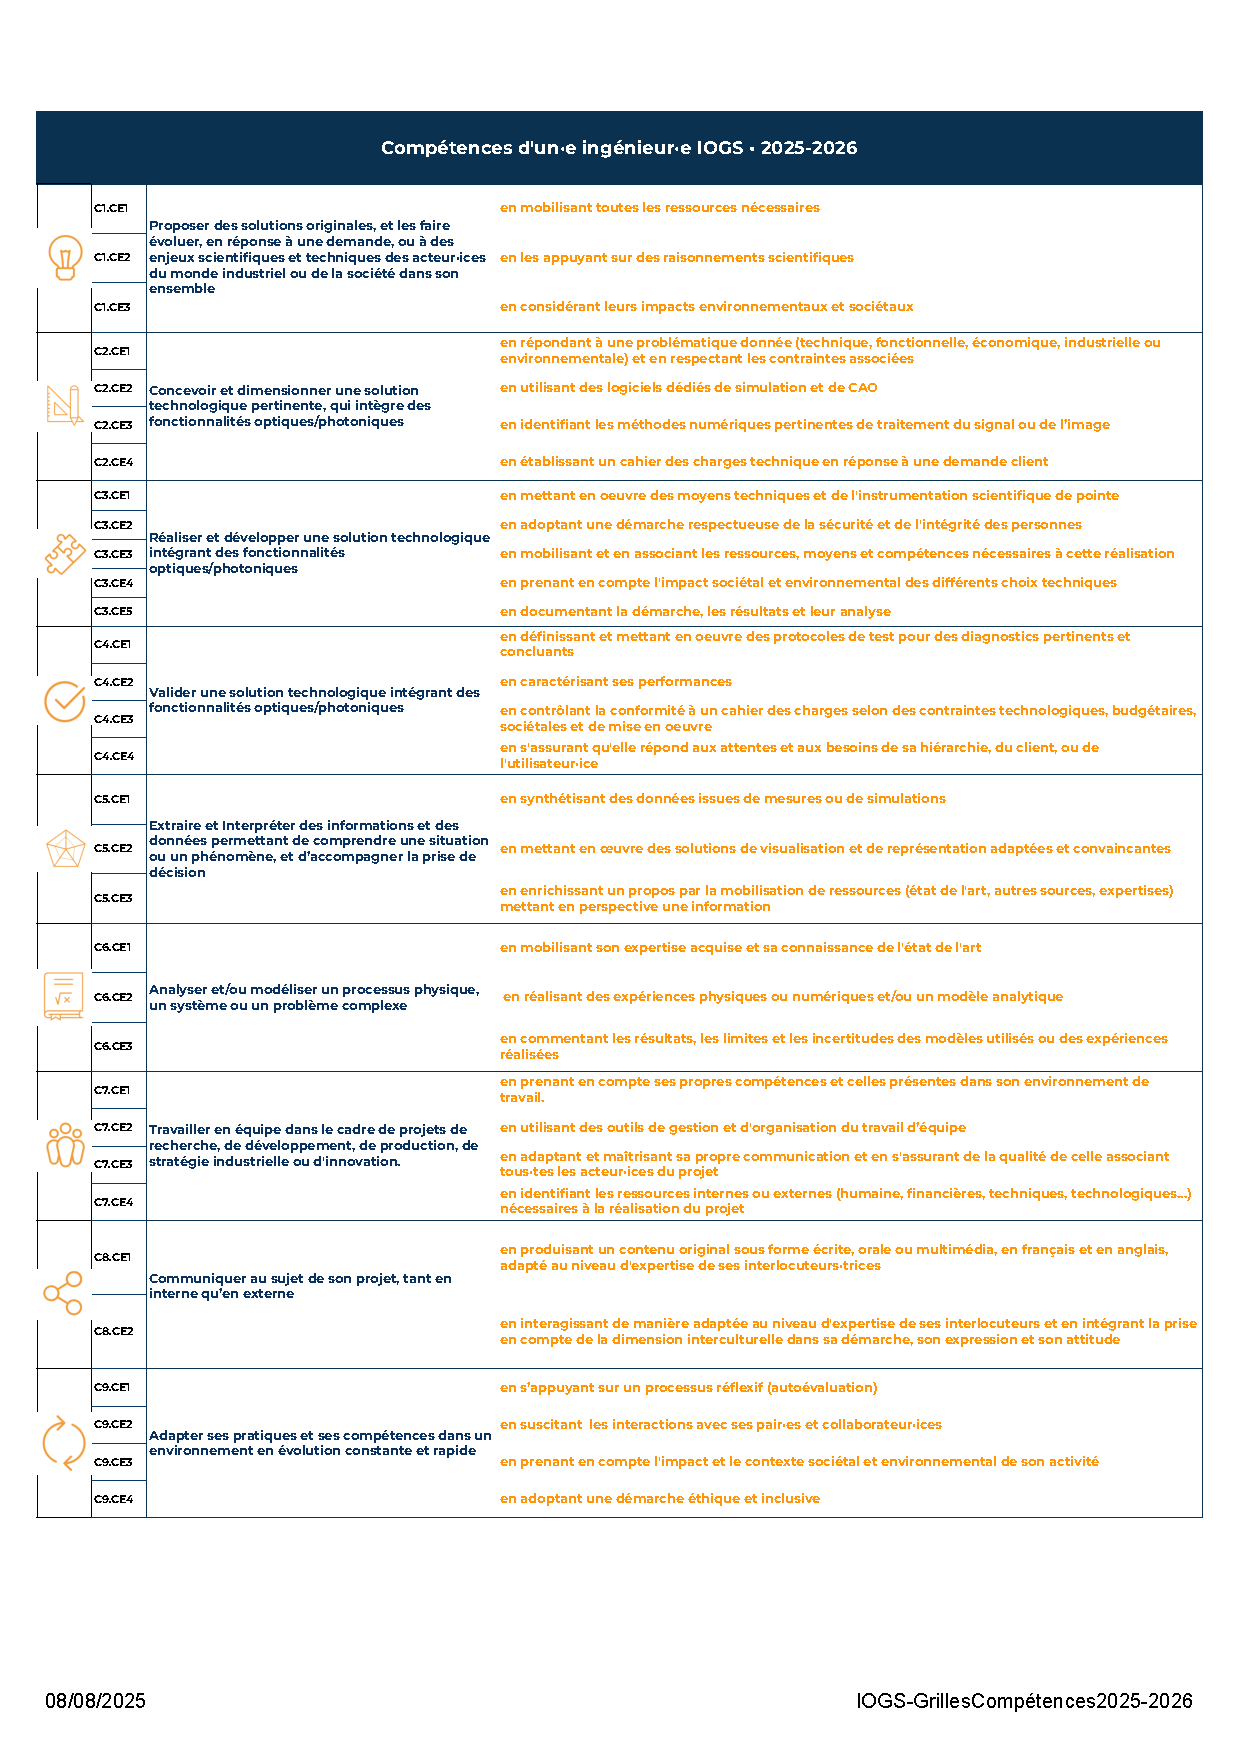
\includepdf[pages={1,4-6}]{apc/IOGS-GrillesCompétences2025-2026.pdf}

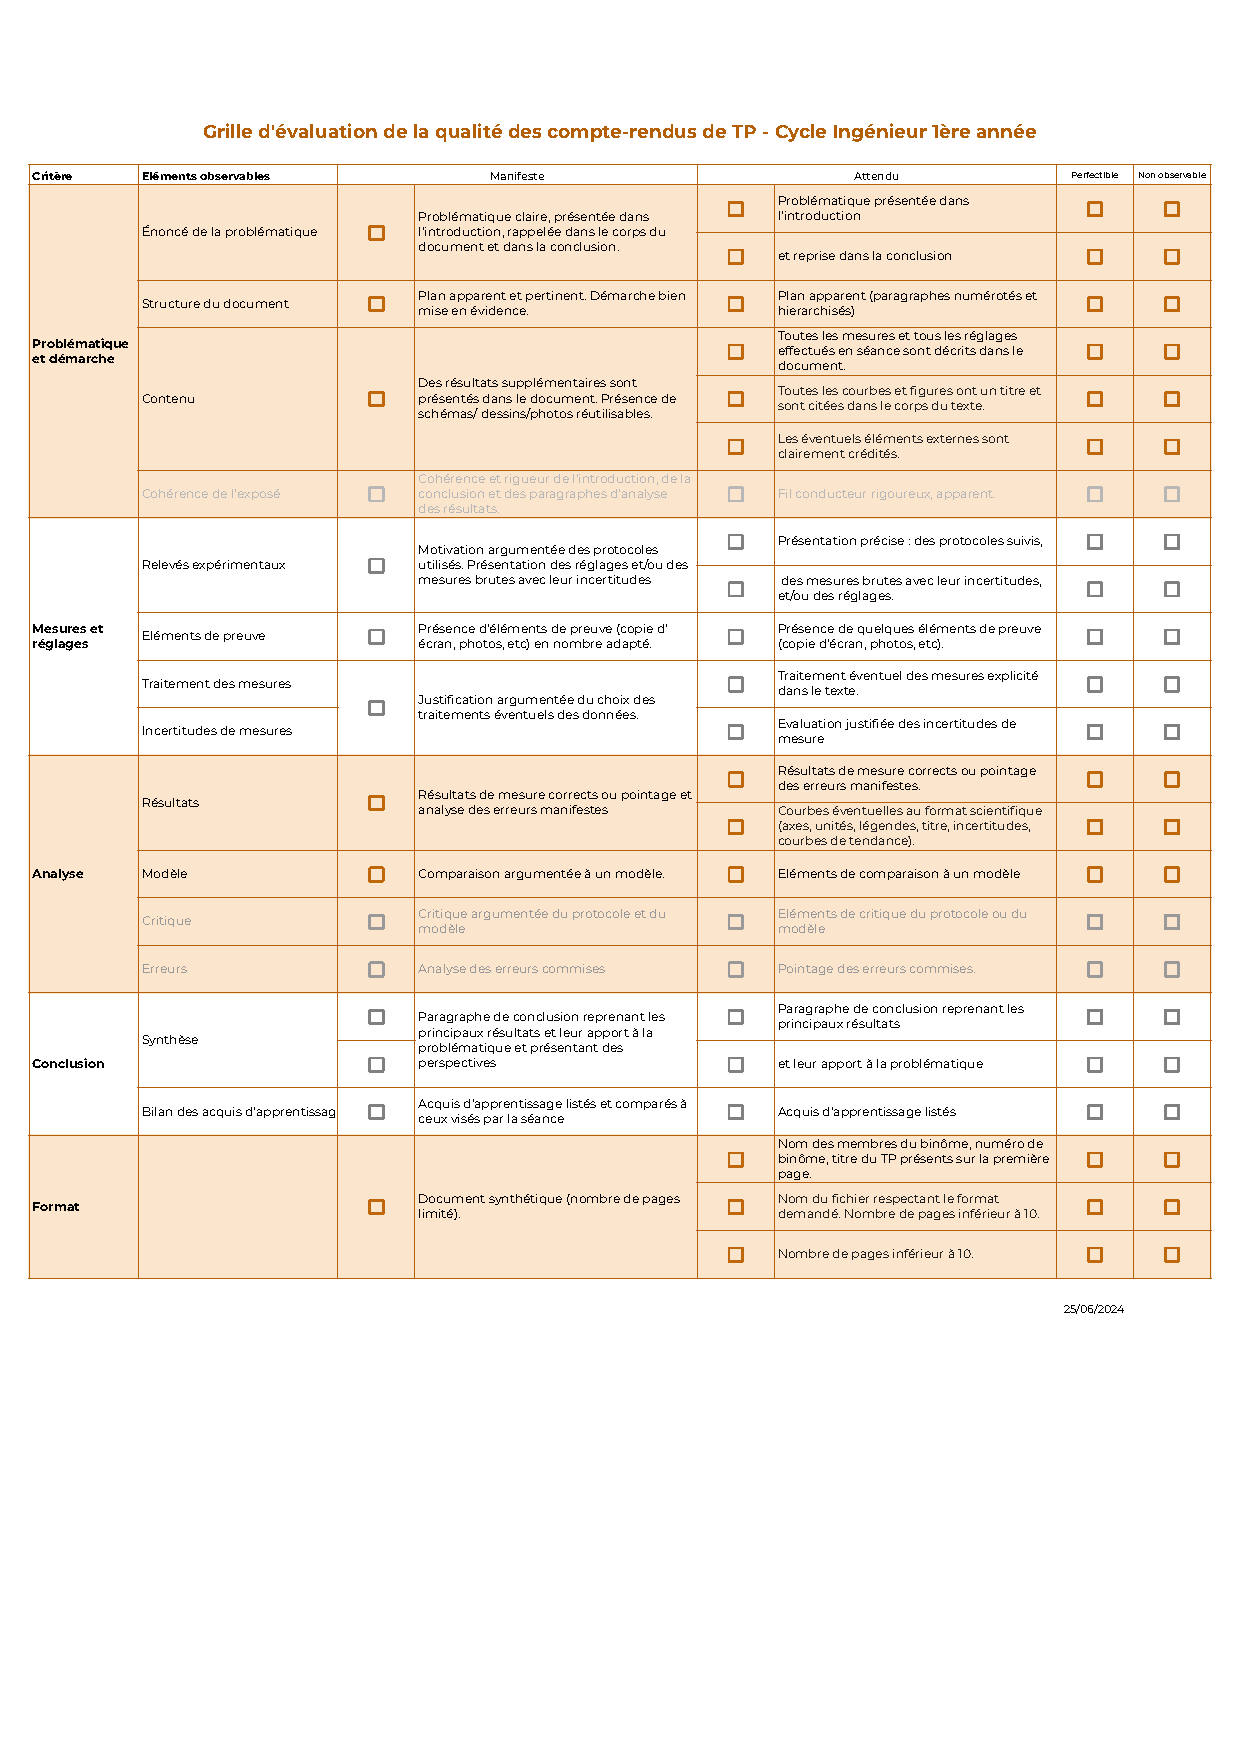
\includepdf[pages=-]{apc/GrillesCRs-1A.pdf}
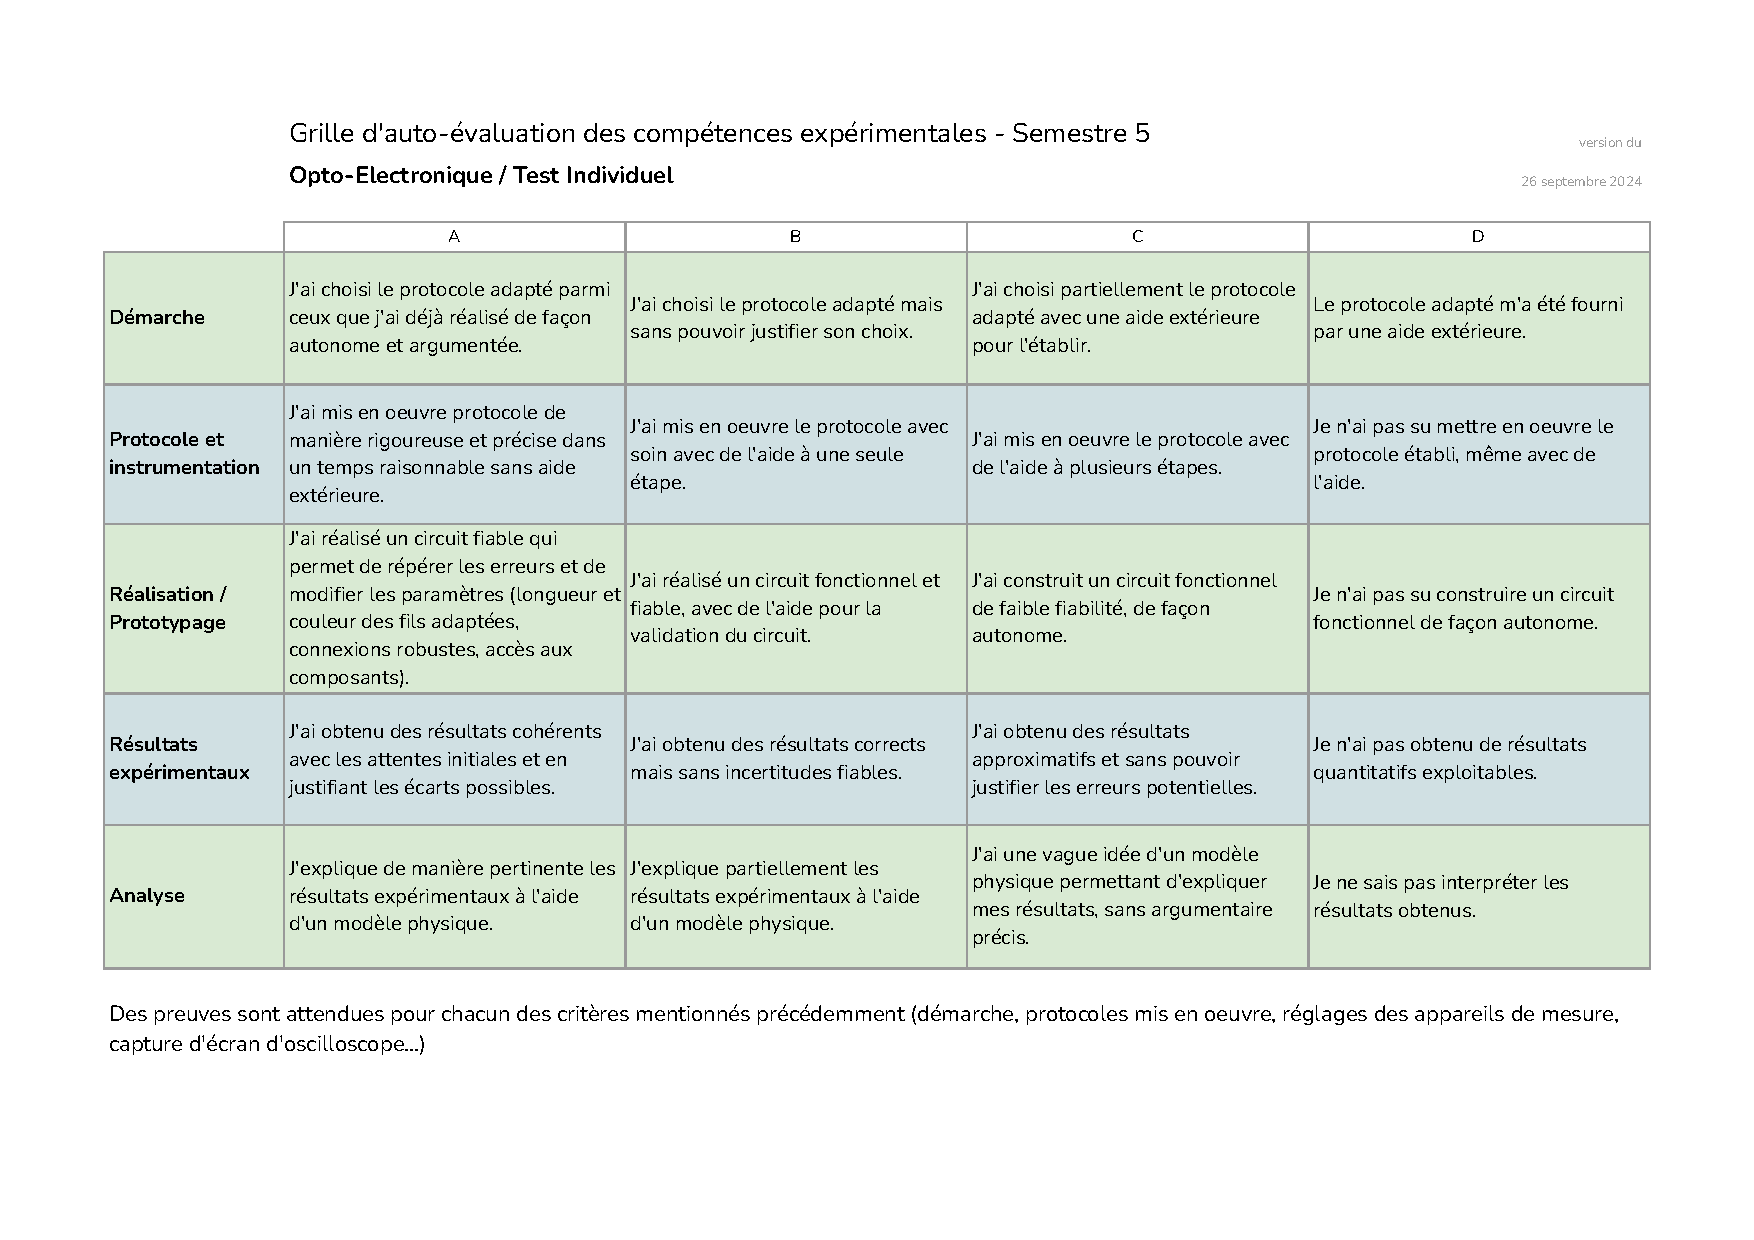
\includepdf[pages=-,landscape=true]{apc/S5_Optoelectronique_2024_AutoEval_Indiv.pdf}

\end{document}


